Laut \S 2 Nr. 8 SigG können Zertifizierungsstellen von natürlichen und juristischen Personen betrieben werden. Der Betrieb einer Zertifizierungsstelle ist grundsätzlich genehmigungsfrei, obliegt dennoch folgenden Bestimmungen nach \S 4 SigG. Man benötigt zum Betrieb Fachkunde, Zuverlässigkeit, Deckungsvorsorge gemäß \S 12 SigG gegen Schadenersatzansprüche sowie Erfüllung der Sicherheitsansprüche anhand eines von der Prüfstelle abgenommenen Sicherheitskonzepts. Die erforderliche Fachkunde liegt vor, wenn die im Betrieb eines Zertifizierungsdienstes tätigen Personen über die für diese Tätigkeit notwendigen Kenntnisse, Erfahrungen und Fertigkeiten verfügen. Die erforderliche Zuverlässigkeit besitzt, wer die Gewähr dafür bietet, als Zertifizierungsdiensteanbieter die für den Betrieb maßgeblichen Rechtsvorschriften einzuhalten. Als Trust Center bezeichnet man die Einrichtungen, die die Verschlüssung von Daten anbieten sowie das Hochsicherheitsrechenzentrum betreiben. Zertifizierungsstellen und Trust Center werden benötigt, wenn eine große Anzahl von Benutzern am digitalen Signaturverfahren teilnehmen. Die Hauptaufgabe der Zertifizierungsstelle ist die Identifizierung der Antragssteller für einen Signaturschlüssel mittels Personalausweis sowie die Vergabe und Zuordnung der öffentlichen Signaturschlüssel. Desweiteren sichern sie die Authentizität des Absenders im Rechtsverkehr, vergleichbar einer amtlichen Beglaubigungen von Behörden und Notaren. \cite{zertstelle1}\cite{standdeswissens3} 
\begin{figure}[!ht]
    \centering
    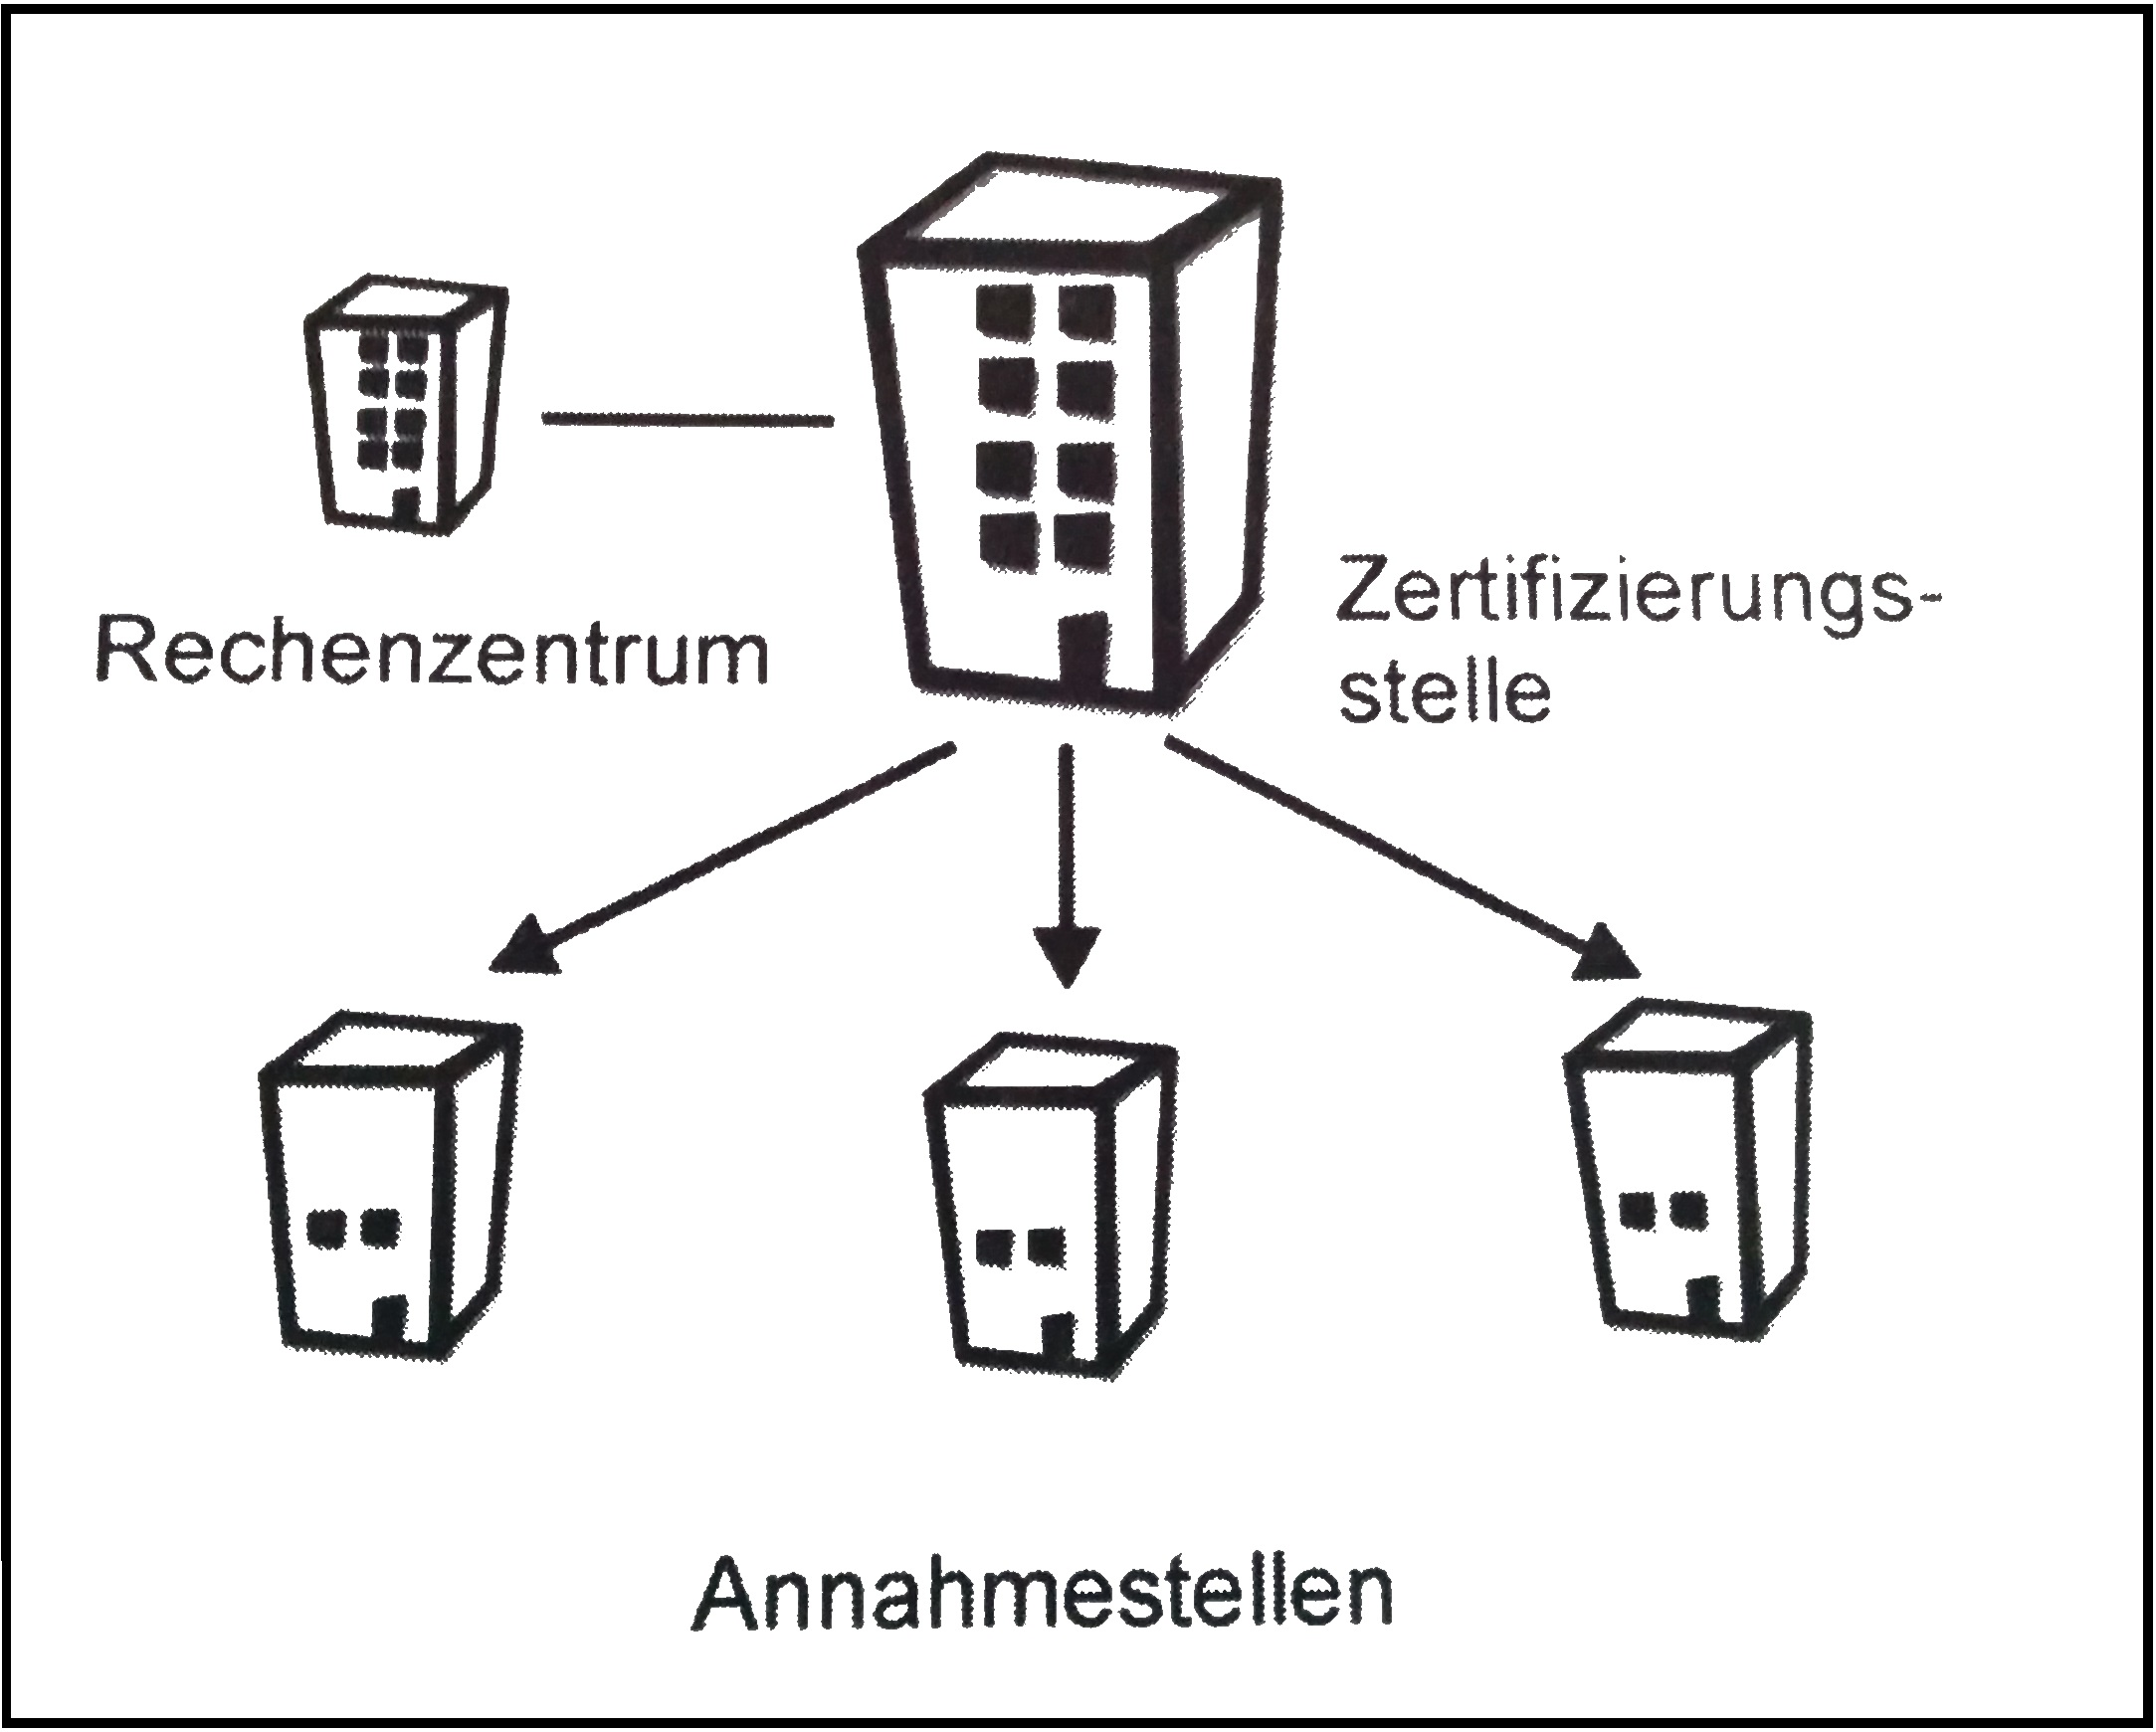
\includegraphics[height=250pt, width=300pt]{trustcenterNeu3.jpg}
    \caption[Schema einer Zertifizierungsstellen]{Schema einer Zertifizierungsstellen. \cite{trust1}}
    \label{fig:1}
\end{figure}\\
Wie auf der Grafik zu sehen ist, lässt sich die Zertifizierungsstelle in 2 Bereiche einteilen. Auf der einen Seite steht die Annahmestelle, welche die Identifikation der Antragsteller mit Personalausweis und weiteren notariell beglaubigten Dokumenten, z.B. Zulassungen übernehmen. Auf der anderen Seite steht die Zertifizierungsstelle, welche die Erzeugung der Schlüsselpaare und Zertifikate übernimmt. Die Zertifizierungsstelle muss sicherstellen, dass niemand den privaten Schlüssel modifizieren kann sowie der Dienst zur Prüfung der Signaturen immer verfügbar ist. Abgesehen davon muss sichergestellt werden, dass nur der Antragsteller den privaten Schlüssel erhält. Dies wird meistens realisiert, indem sich der private Schlüssel unveränderbar auf Chipkarten befindet und nicht ausgelesen oder gelöscht werden kann. \cite{zertstelle1}\cite{standdeswissens3}\\
Zusätzlich müssen Zertifizierungsstellen noch Dienste, wie Zeitstempeldienst, Zulassung von Pseudonyme zur Wahrung des Personlichkeitsrechts des Schlüsselinhabers, Schlüsselverzeichnispflege, 24-Stunden-Sperrdienst für Signaturschlüssel und die Schlüsselaufbewahrung, wenn vom Auftraggeber ausdrücklich gewünscht, ansonsten ist die Speicherung von privaten Schlüsseln nicht erlaubt, anbieten. Der Zeitstempeldienst dient zur genauen Festhaltung, wann ein Dokument erzeugt, verändert oder gelöscht wurde, mittels Zeitangabe der Zertifizierungsstelle im Hashwert für das signierte Dokument. Anwendung findet dieses Verfahren, wenn gesetzliche Fristen eingehalten und Gültigkeitsdauern festgelegt werden sollen. Die Pflege des Schlüsselverzeichnis ist von besonderer Bedeutung, da jederzeit die Identifikation von Kommunikationspartnern möglich sein muss. Das Schlüsselverzeichnis muss ständig aktuell und funktionstüchtig sein.